% !TEX root = main.tex 

\begin{frame}
\frametitle{$\CUT(n)$ and $\COR(n)$ Polytopes}
\onslide<1->{
\begin{definition}[cut polytope]
Let $K_n = (V,E)$ be the complete graph on $n$ vertices. Let $\delta(S)$ denote the cut of $S \subseteq V$. Then let $\chi^{\delta(S)} \in \R^{\abs{E}}$ such that
\[
\chi^{\delta(S)}_e =
\begin{cases}
1 & e \in \delta(S) \\
0 & e \notin \delta(S)
\end{cases}.
\]
Then $\CUT(n) \coloneqq \conv\left( \left\{ \chi^{\delta(S)} \in \R^{\abs{E}} \mid S \subseteq V \right\} \right)$
\end{definition}
}
\onslide<2->{
\begin{definition}[correlation polytope]
We have $\COR(n) \coloneqq \conv\left( \left\{ bb^T \in \R^{n \times n} \mid b \in {\{0, 1\}}^n \right\} \right)$
\end{definition}
}
\end{frame}

\begin{frame}
\frametitle{Connection Between $\CUT(n)$ and $\COR(n)$}
\onslide<1->{
\begin{definition}[linearly isomorphic polytopes]\label{def:lin-iso}
Two polytopes $P \subseteq \R^n$ and $Q \subseteq \R^m$ are called \textit{linearly isomorphic} if there exists a linear invertible function $f : \R^n \to \R^m$ such that $f(P) = Q$.
\end{definition}
}
\onslide<2->{
\begin{lemma}[De Simone, '90]
For all $n$, $\COR(n)$ is linearly isomorphic to $\CUT(n+1)$.
\end{lemma}
}

\onslide<3->{
\begin{corollary}
$\xc(\COR(n)) = \xc(\CUT(n+1))$.
\end{corollary}
}
\end{frame}

\begin{frame}
\frametitle{$\CUT(n)$ has Exponential Extension Complexity}

\onslide<1->{
\begin{theorem}
The extension complexity of $\CUT(n)$ is $2^{\Omega(n)}$.
\end{theorem}
}

\onslide<2->{
\onslide
\begin{proofsketch}
\begin{enumerate}
\item<2-> $\xc(\COR(n)) = \xc(\CUT(n+1))$ 
\item<3-> $\xc(\COR(n)) = \nrank(S)$ where $S$ is the slack matrix of $\COR(n)$
\item<4-> $\nrank(S) \ge \nrank(M)$ 
\item<5-> $\nrank(M) = 2^{\Omega(n)}$.
\end{enumerate}
\vspace{-4mm}
\end{proofsketch}
}

\end{frame}

\begin{frame}
\frametitle{Reductions}
\begin{lemma}
Let $P$ and $F$ be polytopes. If $F$ is a face of $P$, then $\xc(P) \ge \xc(F)$.
\end{lemma}
\end{frame}

\begin{frame}
\frametitle{$\STAB(G)$ Reduces to $\COR(n)$}
\begin{definition}[Stable Set Polytope]
The \emph{stable set polytope} $\STAB(G)$ is defined as the convex hull of the characteristic vectors of all stable sets in $G = (V, E)$. That is,
\[
\STAB(G) \coloneqq \conv\left(\left\{\chi^S \in \R^V \mid S \text{ is a stable set of $G$}\right\}\right).
\]
\end{definition}
\end{frame}

\begin{frame}
\frametitle{Reduction from $\STAB(G)$ to $\COR(n)$}
\begin{itemize}
\item<1-> We will construct a graph $H_n$
\item<2-> Let $K_n$ be the complete graph on the vertices $[n]$
\item<3-> For an edge $\{i,j\}$ in $K_n$ where $i < j$, label the edge $ij$
\item<4-> The vertex set of $H_n$ is
\[
V = \{ii, \ol{ii} : i \in [n]\} \cup \{ij, \ol{ij}, \ul{ij}, \oul{ij}, : i,j \in [n], i < j\}.
\]
\end{itemize}
\end{frame}

\begin{frame}
\frametitle{Reduction from $\STAB(G)$ to $\COR(n)$ (cont.)}
\begin{figure}
\centering
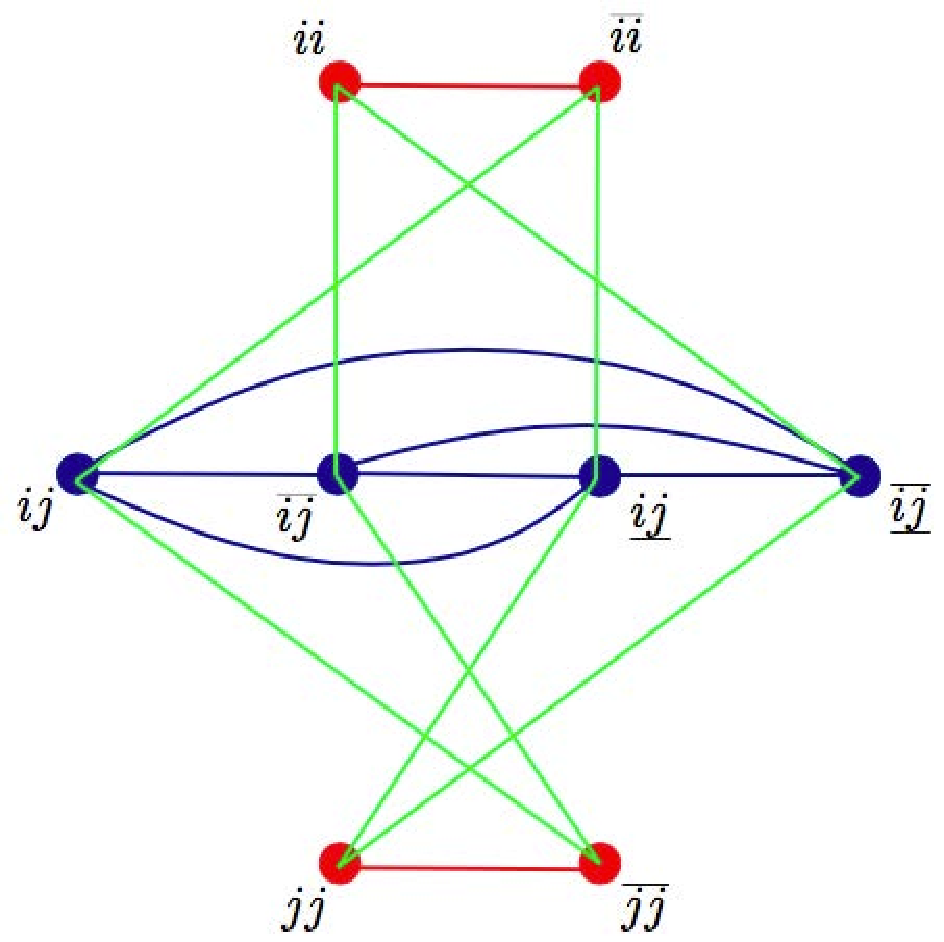
\includegraphics[scale=0.35]{stable.pdf}
\caption{the set of edges and vertices added to $H_n$ for some $i,j \in [n]$ with $i < j$.}
\end{figure}
\end{frame}

\begin{frame}
\frametitle{Reduction from $\STAB(G)$ to $\COR(n)$ (cont.)}

\begin{lemma}
$\STAB(H_n)$ contains a face that is an extension of $\COR(n)$.
\end{lemma}
\end{frame}

\begin{frame}
\frametitle{Extension Complexity of $\STAB(G)$ is $2^{\Omega(\sqrt{n})}$}

\onslide<1->{
\begin{theorem}
For all $n$, there exists a graph $G_n$ with $n$ vertices such that $\xc(\STAB(G_n)) = 2^{\Omega(\sqrt{n})}$.
\end{theorem}
}

\onslide<2->{
\onslide
\begin{proofsketch}
\begin{enumerate}
\item<2-> Let $G_n$ be $H_\ell$ with $n - O(\ell^2)$ isolated vertices \onslide<3->{$\Rightarrow \ell = \Omega(\sqrt{n})$}
\item<4-> $\xc(\STAB(G_n)) \ge \xc(\STAB(H_\ell))$ 
\item<5-> $\xc(\STAB(H_\ell)) \ge \xc(\COR(\ell))$
\item<6-> $ \xc(\COR(\ell)) = 2^{\Omega(\ell)}$
\item<7-> $2^{\Omega(\ell)} = 2^{\Omega(\sqrt{n})}$.
\end{enumerate}
\vspace{-4mm}
\end{proofsketch}
}
\end{frame}




